\chapter{Programmation}
\label{chap:programmation}

La plupart des scripts étant conçu pour fonctionner dans AICA Studio et donc \gls{ros2}, il a été nécessaire d'adopter une architecture spécifique pour permettre la communication entre les différents éléments du système. Toutefois, l'objectif du travail n'était pas d'approfondir la compréhension ou la maîtrise de \gls{ros2} en tant que telle.

Ainsi, la plupart des programmes et blocs fonctionnels ont d'abord été développés et testés en Python de façon indépendante, sans intégration directe à AICA Studio. Cette approche a permis de valider les algorithmes et le fonctionnement général dans un environnement plus simple et maîtrisé.

Dans un second temps, quand le développement a été finalisé, l'intégration dans l'environnement AICA Studio a été réalisée. Cette étape a consisté à adapter les scripts pour qu'ils fonctionnent avec l'architecture \gls{ros2} imposée par AICA Studio, en veillant à la compatibilité des communications et à l'intégration des blocs fonctionnels dans le système global.

Cette démarche a permis de gagner du temps sur le développement initial, tout en assurant une intégration robuste et conforme aux exigences de la plateforme finale.

\section{Ecran tactile}
L'écran tactile ED101 est le seul élément de la maquette qui n'est pas directement lié au logiciel AICA Studio. Un script Python a été développé avec la bibliothèque \texttt{tkinter} pour permettre à l'utilisateur de dessiner et d'envoyer directement le fichier DXF correspondant au PC principal. Un Bloc fonctionnel a été créé dans AICA Studio pour recevoir ce fichier DXF.

\begin{figure}[H]
    \centering
    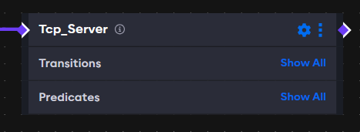
\includegraphics[width=0.8\textwidth]{assets/figures/AICA_Tcp_Server.png}
    \caption{Bloc fonctionnel du serveur TCP dans AICA Studio}
    \label{fig:touchscreen_interface}
\end{figure}

\section{Graveuse laser}
Afin de pouvoir communiquer avec la graveuse laser depuis le logiciel AICA Studio, un bloc fonctionnel a été développé afin de :
\begin{itemize}
    \item Charger un fichier DXF.
    \item Convertir le fichier DXF en G-code.
    \item Envoyer le G-code à la graveuse laser.
    \item Gérer la synchronisation entre le bras robot et la graveuse laser.
\end{itemize}

\begin{figure}[H]
    \centering
    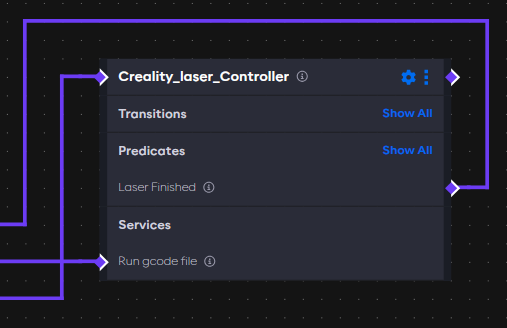
\includegraphics[width=0.8\textwidth]{assets/figures/AICA_Laser_interface.png}
    \caption{Bloc fonctionnel de la graveuse laser dans AICA Studio}
    \label{fig:laser_interface}
\end{figure}

Le bloc fonctionnel offre une certaine liberté dans le choix du nom du fichier DXF. Cependant, dans le cadre du projet, le nom de fichier est toujours le même. Le script de récupération s'occupe de remplacer le fichier quand un plus récent est reçu.

\section{Caméra}

La caméra Intel D435 est intégrée dans le système via un bloc fonctionnel personnalisé développé dans AICA Studio. Ce bloc utilise les données de profondeur captées par la caméra pour détecter la position des pièces à graver et adapter la trajectoire du bras robot en conséquence.
Afin d'obtenir un retour de données rapide, le code est optimisé pour minimiser le temps de traitement et permettre une mise a jour toutes les 300ms. Le but est d'envoyer le robot à la position de la pièce à prendre et de corriger la trajectoire toutes les 300ms.
Le programme fonctionne selon les étapes suivantes :
\begin{figure}[H]
    \centering
    \begin{minipage}{0.55\textwidth}
        \centering
        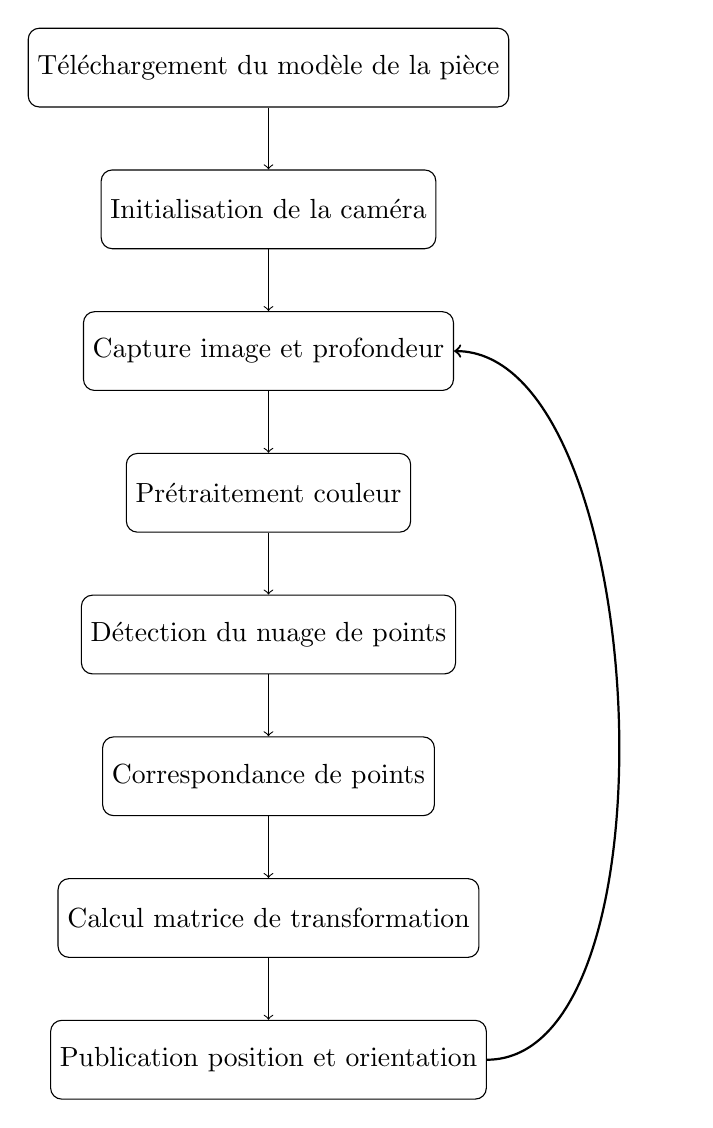
\begin{tikzpicture}[node distance=1.8cm, every node/.style={draw, align=center, rounded corners, minimum height=1cm}]

            \node (load) {Téléchargement du modèle de la pièce};
            \node (init) [below of=load] {Initialisation de la caméra};
            \node (capture) [below of=init] {Capture image et profondeur};
            \node (preprocess) [below of=capture] {Prétraitement couleur};
            \node (cloud) [below of=preprocess] {Détection du nuage de points};
            \node (match) [below of=cloud] {Correspondance de points};
            \node (matrice) [below of=match] {Calcul matrice de transformation};
            \node (publish) [below of=matrice] {Publication position et orientation};
            \draw[->] (load) -- (init);
            \draw[->] (init) -- (capture);
            \draw[->] (capture) -- (preprocess);
            \draw[->] (preprocess) -- (cloud);
            \draw[->] (cloud) -- (match);
            \draw[->] (match) -- (matrice);
            \draw[->] (matrice) -- (publish);
            \draw[->, thick] (publish.east) .. controls +(right:2.5cm) and +(right:2.5cm) .. (capture.east);
        \end{tikzpicture}
    \end{minipage}%
    \hfill
    \begin{minipage}{0.4\textwidth}
        \centering
        \begin{subfigure}{0.8\linewidth}
            \fbox{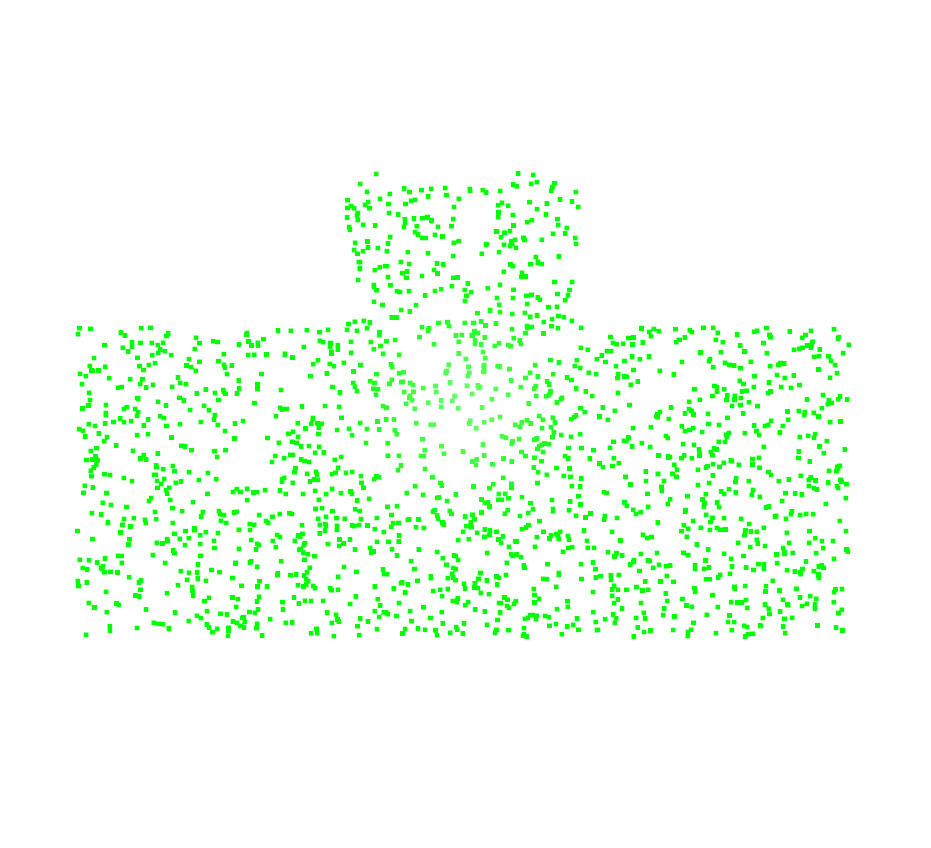
\includegraphics[width=\linewidth]{assets/figures/Piece_model.png}}
            \caption{Modèle 3D de la pièce}
        \end{subfigure}\\[0.2cm]
        \begin{subfigure}{0.8\linewidth}
            \fbox{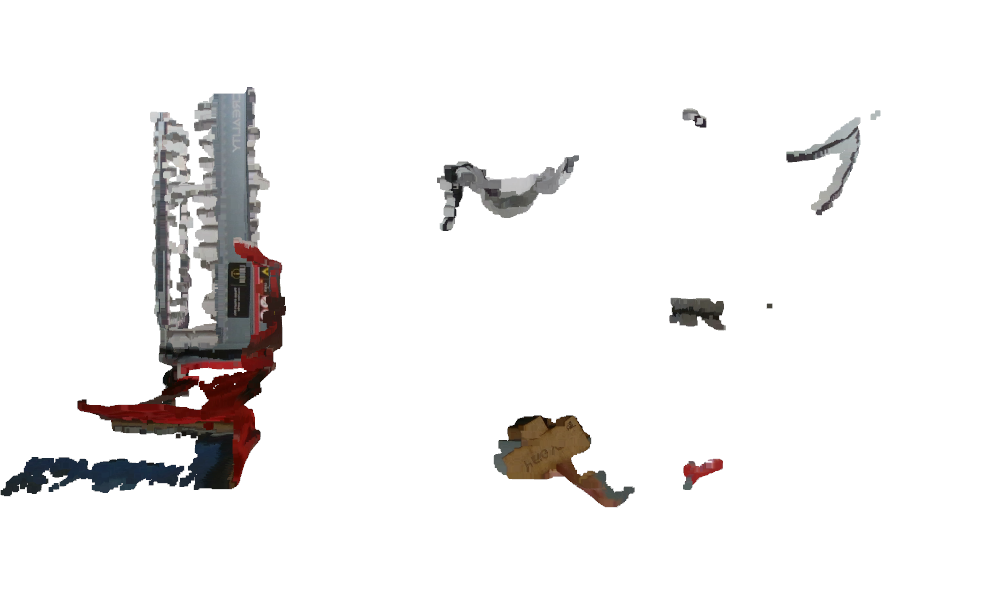
\includegraphics[width=\linewidth]{assets/figures/photo_origin.png}}
            \caption{Prise de la photo}
        \end{subfigure}\\[0.2cm]
        \begin{subfigure}{0.8\linewidth}
            \fbox{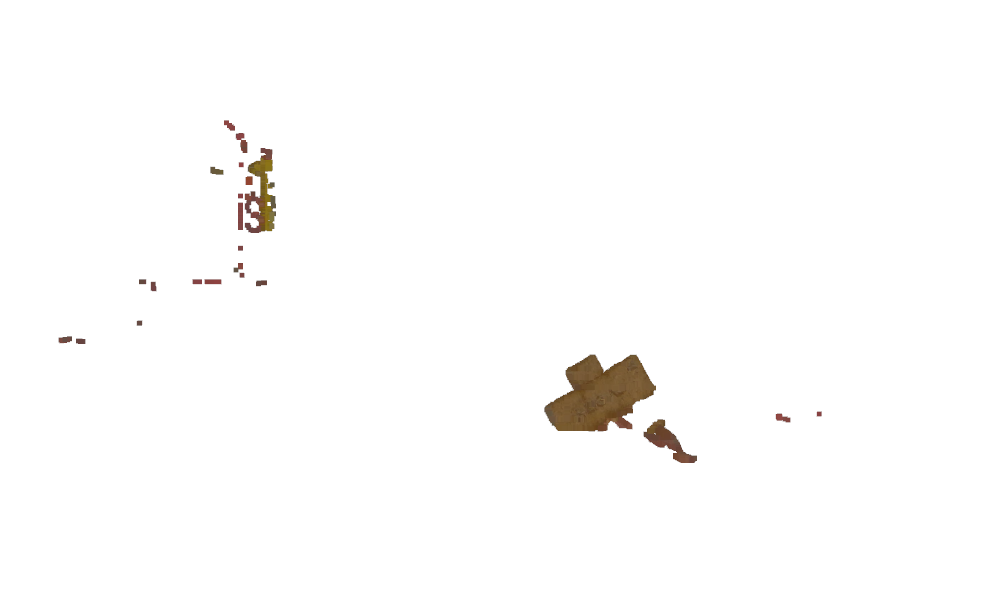
\includegraphics[width=\linewidth]{assets/figures/filtrage_couleur.png}}
            \caption{Filtrage par couleur}
        \end{subfigure}\\[0.2cm]
        \begin{subfigure}{0.8\linewidth}
            \fbox{
\includegraphics[width=\linewidth]{assets/figures/detection_piece.png}}
            \caption{Isolement de la pièce}
        \end{subfigure}\\[0.2cm]
        \begin{subfigure}{0.8\linewidth}
            \fbox{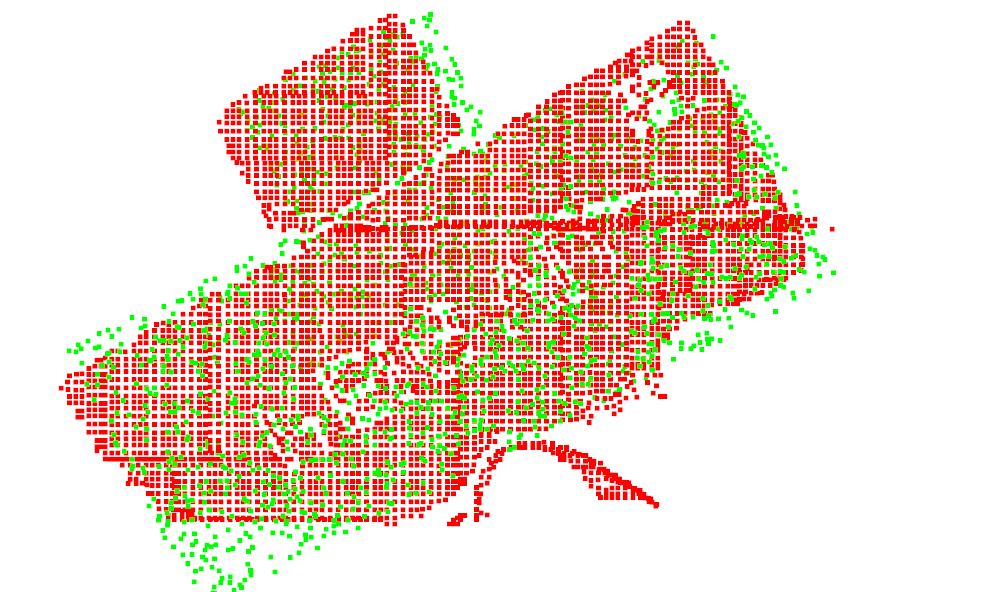
\includegraphics[width=\linewidth]{assets/figures/superposition.png}}
            \caption{Superposition modèle/réalité}
        \end{subfigure}
    \end{minipage}
    \caption{Schéma de séquence du programme de la caméra Intel D435, avec illustrations des étapes principales}
    \label{fig:sequence_camera_illustre}
\end{figure}

Tout comme le bloc fonctionnel de la graveuse laser, le bloc fonctionnel de la caméra offre une certaine liberté dans les paramètres de traitement. Il est par exemple possible de choisir la couleur de la pièce à détecter, modifier le modèle ainsi que le nombre de points de ce dernier. Cette flexibilité permet d'adapter le système tant dans la pièce à détecter que dans la rapidité de traitement.

\begin{figure}[H]
    \centering
    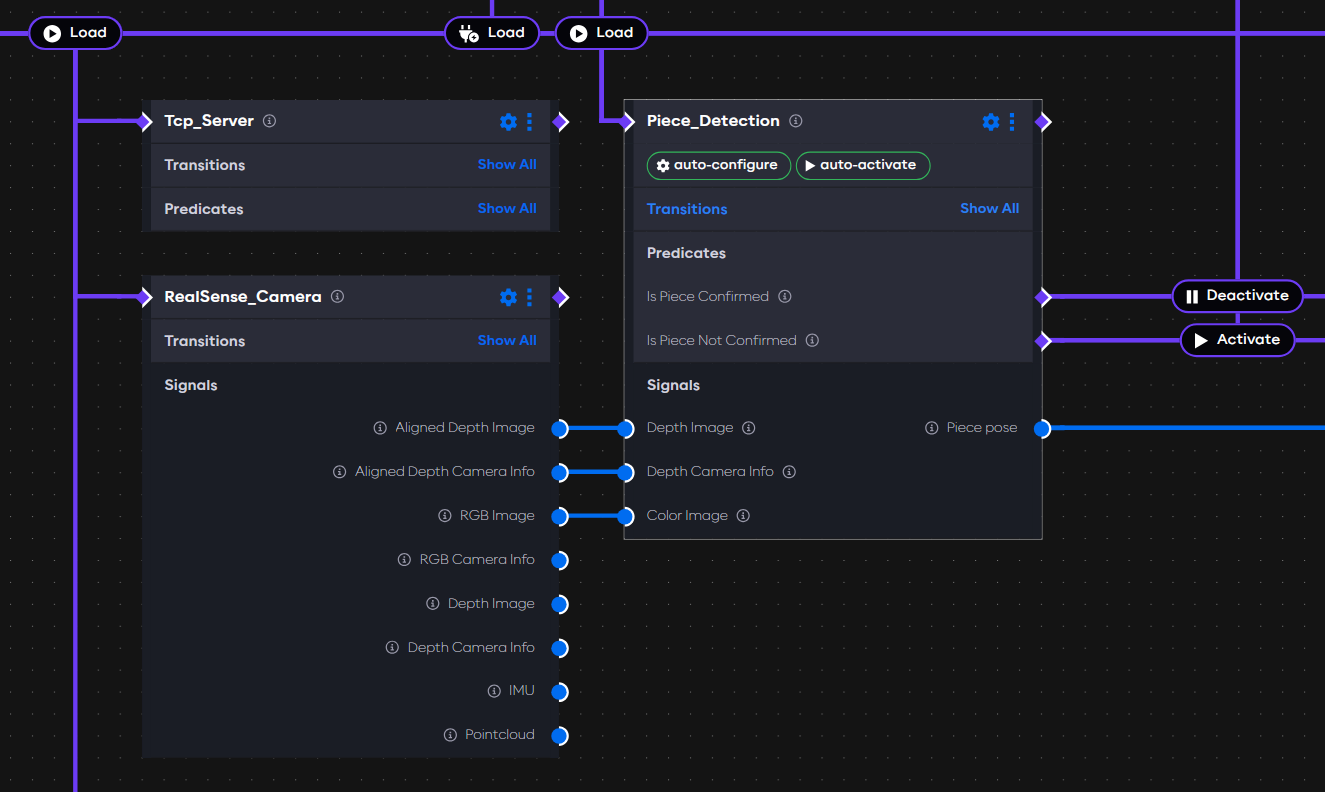
\includegraphics[width=0.8\textwidth]{assets/figures/AICA_Camera.png}
    \caption{Bloc fonctionnel de la caméra dans AICA Studio}
    \label{fig:camera_interface}
\end{figure}

\subsection{Transformation du repère caméra au repère robot}

Pour obtenir la position de la pièce détectée dans le repère du robot (ou du monde), le programme effectue une composition de transformations :

\begin{enumerate}
    \item \textbf{Détection de la pièce dans le repère caméra} :
          \begin{itemize}
              \item La position de la pièce est estimée en superposant le centroïde du modèle 3D (référence) et celui de la pièce détectée dans l'image. Cette position est donc exprimée dans le repère de la caméra.
              \item La rotation de la pièce est déterminée en testant différentes orientations (rotation degré par degré autour de chaque axe) et en cherchant celle qui aligne au mieux le modèle 3D avec la pièce détectée. Cette rotation est également exprimée dans le repère de la caméra.
          \end{itemize}
    \item \textbf{Transformation du repère caméra au repère monde (robot)} :
          \begin{itemize}
              \item La position et l'orientation de la caméra dans le repère monde (ou robot) sont connues et définies par une translation et un quaternion (paramètre \texttt{camera\_pose\_world}).
              \item On construit la matrice de transformation homogène de la caméra dans le monde : $T_{\text{cam} \to \text{world}}$.
          \end{itemize}
    \item \textbf{Calcul de la position finale de la pièce dans le monde} :
          \begin{itemize}
              \item On compose la transformation de la pièce dans la caméra ($T_{\text{piece} \to \text{cam}}$) avec celle de la caméra dans le monde ($T_{\text{cam} \to \text{world}}$) :
                    \[
                        T_{\text{piece} \to \text{world}} = T_{\text{cam} \to \text{world}} \cdot T_{\text{piece} \to \text{cam}}
                    \]
              \item On obtient ainsi la position et l'orientation de la pièce dans le repère monde (robot), ce qui permet au robot de s'y rendre précisément.
          \end{itemize}
    \item \textbf{Implémentation dans le code} :
          \begin{itemize}
              \item Le code utilise la librairie \texttt{scipy.spatial.transform.Rotation} pour convertir les quaternions en matrices de rotation, et \texttt{numpy} pour manipuler les matrices de transformation.
          \end{itemize}
\end{enumerate}

Cette méthode permet de publier la position et l'orientation de la pièce dans le repère global, ce qui est indispensable pour que le robot puisse saisir ou interagir avec la pièce détectée.

\subsection{Valeurs de la matrice de transformation}

Dans ce projet, il n'a pas été nécessaire de réaliser une calibration manuelle entre la caméra et le repère robot. En effet, grâce au modèle 3D précis de la maquette, la position et l'orientation de la caméra ont pu être déterminées virtuellement, ce qui a permis de renseigner directement la matrice de transformation dans le programme.

\begin{minipage}{0.55\textwidth}
    \paragraph{Transformation caméra → monde}
    La pose de la caméra dans le monde utilisée dans le code est la suivante :
    \begin{itemize}
        \item Translation (m) : $[0.420451,\ 0.0175,\ 0.766251]$
        \item Quaternion (w, x, y, z) : $[0,\ -0.707107,\ 0.707107,\ 0]$
    \end{itemize}
    {\rowcolors{2}{}{}}%
    La matrice de transformation homogène correspondante est :
    \begin{equation*}
        T_{\text{cam} \to \text{world}} =
        \begin{bmatrix}
            0 & -1 & 0 & 0.420451 \\
           -1 & 0 & 0  & 0.0175   \\
            0 & 0 & -1  & 0.766251 \\
            0 & 0 & 0  & 1
        \end{bmatrix}
    \end{equation*}
    Cette transformation permet de passer des coordonnées caméra aux coordonnées monde (robot), ce qui est indispensable pour la localisation de la pièce par le robot.
\end{minipage}%
\hfill
\begin{minipage}{0.4\textwidth}
    \centering
    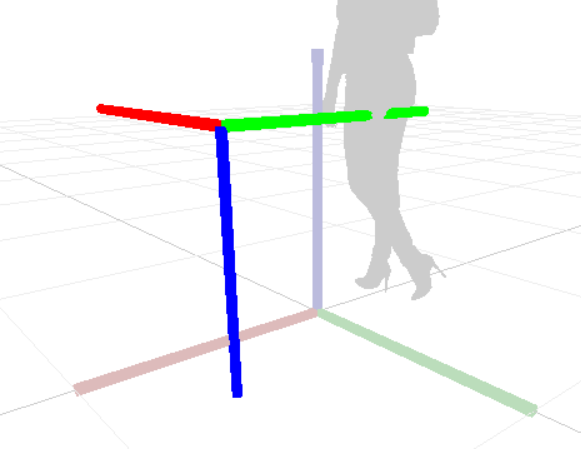
\includegraphics[width=0.95\linewidth]{assets/figures/Transform_example.png}
    \captionof{figure}{Illustration de la transformation de repère caméra vers monde}
\end{minipage}

\section{AICA Studio}
Afin de faire fonctionner les différents blocs fonctionnels développés, il est donc nécessaire de les intégrer dans AICA Studio. A l'aide de blocs de base du logiciel et de certains blocs fournis après coup par l'entreprise, il a été possible de créer un programme qui relie tous les éléments de la maquette ensemble.
\begin{figure}[H]
    \centering
    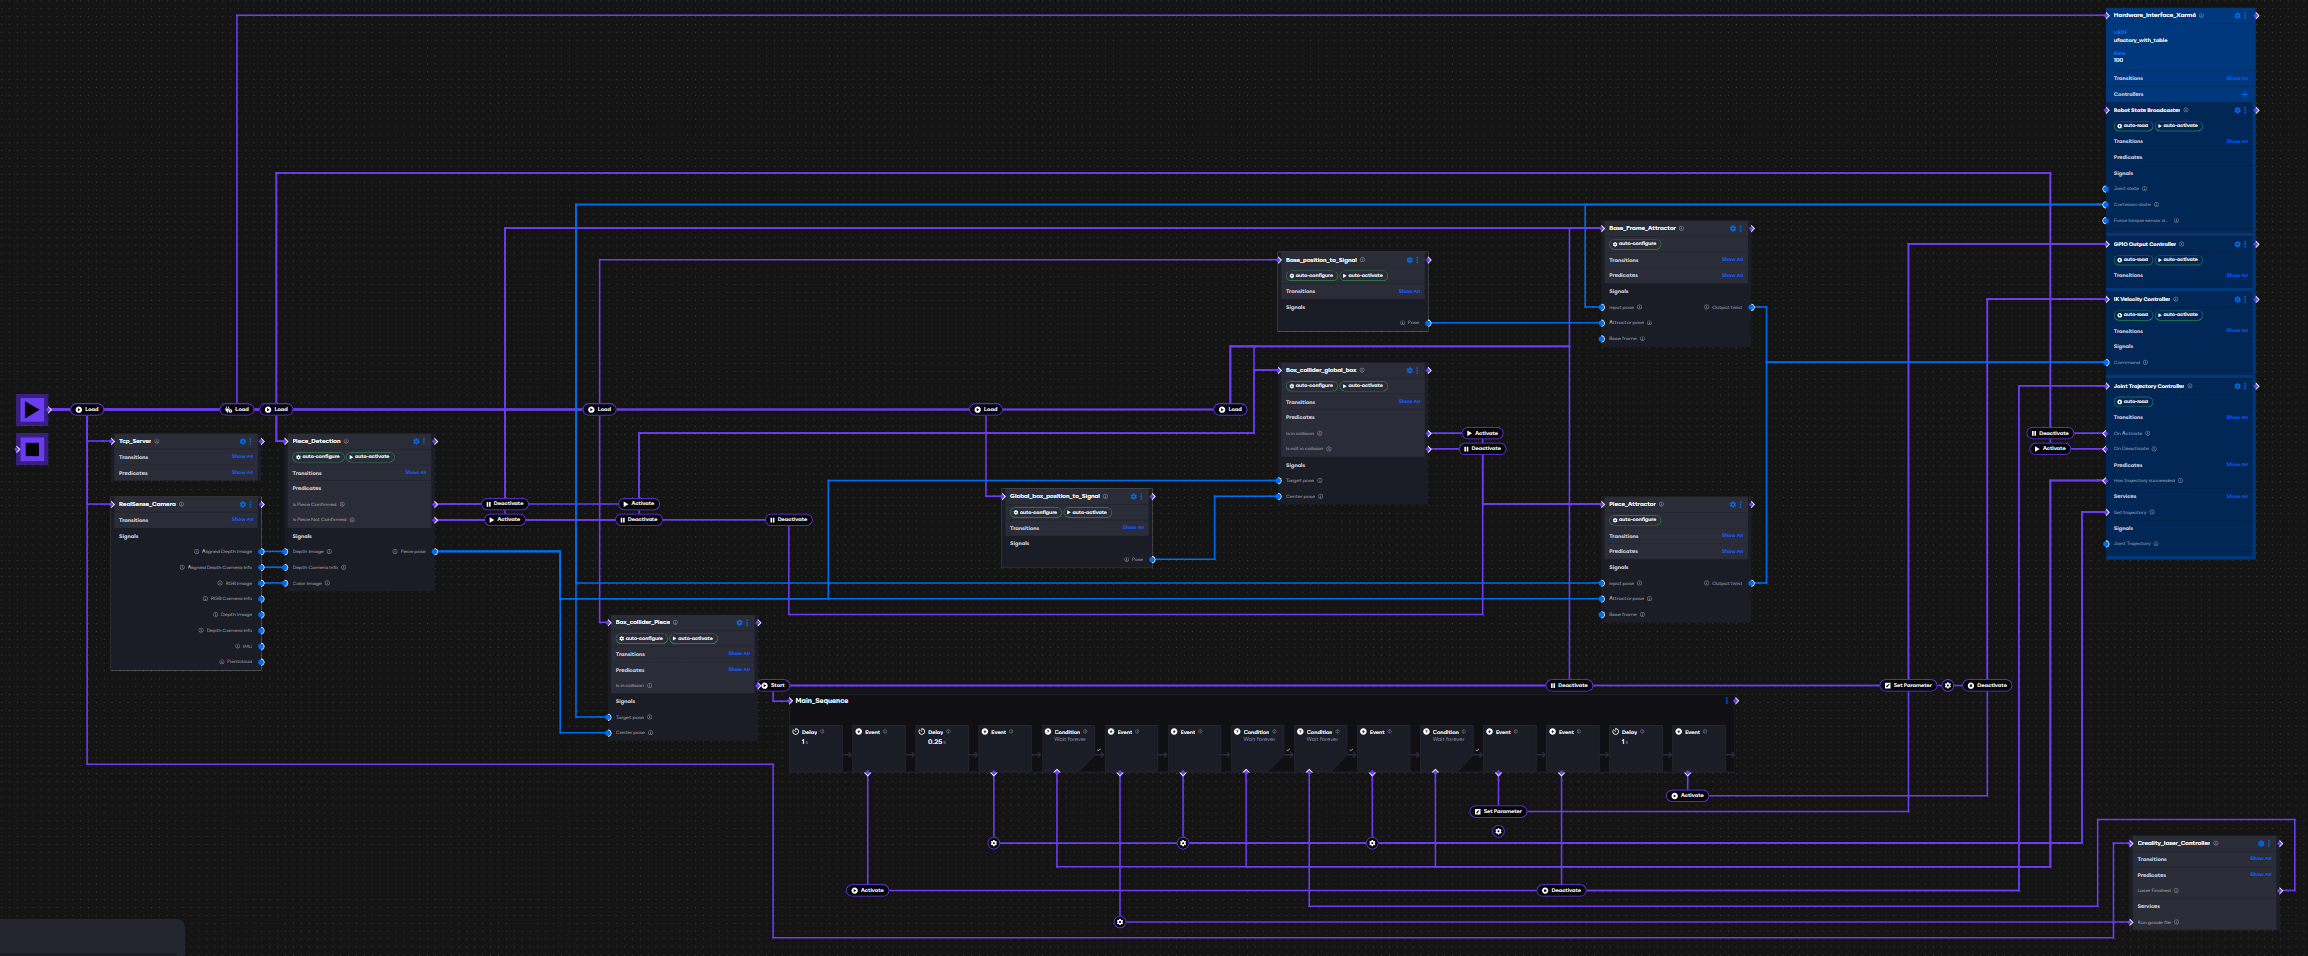
\includegraphics[width=0.8\textwidth]{assets/figures/AICA_Prog_All.png}
    \caption{Programme AICA Studio de la maquette de la graveuse laser intelligente}
    \label{fig:aica_programme}
\end{figure}


